\documentclass[a4paper]{article}
\usepackage[ngerman]{babel}
\usepackage[utf8]{inputenc}
\usepackage{multicol}
\usepackage{calc}
\usepackage{ifthen}
\usepackage[landscape]{geometry}
\usepackage{amsmath,amsthm,amsfonts,amssymb}
\usepackage{color,graphicx,overpic}
\usepackage{xcolor, listings}
\usepackage{textcomp}
\usepackage[compact]{titlesec} %less space for headers
\usepackage{mdwlist} %less space for lists
\usepackage{pdflscape}
\usepackage{verbatim}
\usepackage[hidelinks,pdfencoding=auto]{hyperref}
\usepackage{fancyhdr}
\usepackage{lastpage}
\pagestyle{fancy}
\fancyhf{}
\fancyhead[L]{Datenbanksysteme}
\fancyfoot[L]{\thepage/\pageref{LastPage}}
\renewcommand{\headrulewidth}{0pt} %obere Trennlinie
\renewcommand{\footrulewidth}{0pt} %untere Trennlinie

\pdfinfo{
    /Title (Datenbanksysteme - Cheatsheet)
    /Creator (TeX)
    /Producer (pdfTeX 1.40.0)
    /Author (Robert Jeutter)
    /Subject ()
}

%%% Code Listings
\definecolor{codegreen}{rgb}{0,0.6,0}
\definecolor{codegray}{rgb}{0.5,0.5,0.5}
\definecolor{codepurple}{rgb}{0.58,0,0.82}
\definecolor{backcolour}{rgb}{0.95,0.95,0.92}
\lstdefinestyle{mystyle}{
  backgroundcolor=\color{backcolour},   
  commentstyle=\color{codegreen},
  keywordstyle=\color{magenta},
  numberstyle=\tiny\color{codegray},
  stringstyle=\color{codepurple},
  basicstyle=\ttfamily,
  breakatwhitespace=false, 
}
\lstset{style=mystyle, upquote=true}

% This sets page margins to .5 inch if using letter paper, and to 1cm
% if using A4 paper. (This probably isn"t strictly necessary.)
% If using another size paper, use default 1cm margins.
\ifthenelse{\lengthtest { \paperwidth = 11in}}
    { \geometry{top=.5in,left=.5in,right=.5in,bottom=.5in} }
    {\ifthenelse{ \lengthtest{ \paperwidth = 297mm}}
    {\geometry{top=1.3cm,left=1cm,right=1cm,bottom=1.2cm} }
    {\geometry{top=1.3cm,left=1cm,right=1cm,bottom=1.2cm} }
    }

% Redefine section commands to use less space
\makeatletter
\renewcommand{\section}{\@startsection{section}{1}{0mm}%
                                {-1ex plus -.5ex minus -.2ex}%
                                {0.5ex plus .2ex}%x
                                {\normalfont\large\bfseries}}
\renewcommand{\subsection}{\@startsection{subsection}{2}{0mm}%
                                {-1explus -.5ex minus -.2ex}%
                                {0.5ex plus .2ex}%
                                {\normalfont\normalsize\bfseries}}
\renewcommand{\subsubsection}{\@startsection{subsubsection}{3}{0mm}%
                                {-1ex plus -.5ex minus -.2ex}%
                                {1ex plus .2ex}%
                                {\normalfont\small\bfseries}}
\makeatother

% Define BibTeX command
\def\BibTeX{{\rm B\kern-.05em{\sc i\kern-.025em b}\kern-.08em
    T\kern-.1667em\lower.7ex\hbox{E}\kern-.125emX}}

% Don"t print section numbers
\setcounter{secnumdepth}{0}

\setlength{\parindent}{0pt}
\setlength{\parskip}{0pt plus 0.5ex}    
% compress space
\setlength\abovedisplayskip{0pt}
\setlength{\parskip}{0pt}
\setlength{\parsep}{0pt}
\setlength{\topskip}{0pt}
\setlength{\topsep}{0pt}
\setlength{\partopsep}{0pt}
\linespread{0.5}
\titlespacing{\section}{0pt}{*0}{*0}
\titlespacing{\subsection}{0pt}{*0}{*0}
\titlespacing{\subsubsection}{0pt}{*0}{*0}

\begin{document}

\raggedright
\begin{multicols}{3}
    \scriptsize
    % multicol parameters
    % These lengths are set only within the two main columns
    %\setlength{\columnseprule}{0.25pt}
    \setlength{\premulticols}{1pt}
    \setlength{\postmulticols}{1pt}
    \setlength{\multicolsep}{1pt}
    \setlength{\columnsep}{2pt}

    \section{SQL}
    \begin{lstlisting}[
        language=SQL,
        showspaces=false,
        basicstyle=\ttfamily,
        commentstyle=\color{gray}
     ]
CREATE TABLE t (
    id INT PRIMARY KEY,
    c1 TEXT,
    name VARCHAR NOT NULL,
    price INT DEFAULT 0,
    PRIMARY KEY (id),
    FOREIGN KEY (c1) REFERENCES t2(c2),
    UNIQUE(id,name), 
    CHECK(id> 0 AND price >= id)
);

DROP TABLE t; //Delete table
ALTER TABLE t ADD column; //Add new column
ALTER TABLE t DROP COLUMN c; //Drop column
ALTER TABLE t ADD constraint; //Add constraint
ALTER TABLE t1 RENAME TO t2; //Rename table
ALTER TABLE t DROP constraint; //Drop constraint
ALTER TABLE t1 RENAME c1 TO c2; //Rename column

INSERT INTO t(column_list) VALUES(value_list);
...SELECT column_list FROM t2;
UPDATE t SET c1= new_value;
UPDATE t SET c1 = new_value WHERE condition;
DELETE FROM t; //Delete all data
DELETE FROM t WHERE condition; //Delete subset

SELECT c1, c2 FROM t //Query data
SELECT c1, c2 FROM t1, t2 //cross join
SELECT * FROM t //Query all rows
SELECT DISTINCT... //Query distinct rows
    ...UNION [ALL] //Combine rows from queries
    ...INTERSECT //Return intersection
    ...MINUS //Subtract result

...WHERE condition //with condition
    ...IS [NOT] NULL
    ...[NOT] LIKE %xy_ //%=beliebig viele; $=ein Zeichen
    ...[NOT] IN value_list
    ...BETWEEN low AND high

...GROUP BY c1 //Group rows
...GROUP BY c1 HAVING condition; //Filter
...ORDER BY c1 ASC [DESC] //Sort result
...HAVING bedingung // !TODO
...LIMIT n OFFSET offset //return n rows

...INNER JOIN t2 ON condition
...LEFT JOIN t2 ON condition
...RIGHT JOIN t2 ON condition
...FULL OUTER JOIN t2 ON condition
...CROSS JOIN t2 //Cartesian product

CREATE VIEW v(c1,c2) AS SELECT c1, c2 FROM t;
CREATE RECURSIVE VIEW...
CREATE TEMPORARY VIEW... 
...UNION [ALL]
...WITH [CASCADED | LOCAL] CHECK OPTION;
DROP VIEW view_name;

CREATE INDEX idx_name ON t(c1,c2);
CREATE UNIQUE INDEX idx_name ON t(c3,c4);
DROP INDEX idx_name;

CREATE OR MODIFY TRIGGER trigger_name
    [BEFORE | AFTER] [INSERT | UPDATE | DELETE] 
    ON table_name FOR EACH [ROW | STATEMENT]
    EXECUTE stored_procedure;
DROP TRIGGER trigger_name;

CREATE ASSERTION name CHECK (praedikat)
GRANT rechte ON tabelle TO nutzer [with grant option]
REVOKE rechte ON tabelle TO nutzer [restrict | cascade ]

//AGGREGATE FUNCTIONS
AVG     //returns the average of a list
COUNT   //returns the number of elements of a list 
SUM     //returns the total of a list
MAX     //returns the maximum value in a list
MIN     //returns the minimum value in a list
\end{lstlisting}

    \section{NoSQL (MongoDB)}
    \begin{lstlisting}[
        language=SQL,
        showspaces=false,
        basicstyle=\ttfamily,
        commentstyle=\color{gray}
     ]
db.createUser({
    user: "dbadmin",
    pwd: "12345678",
    roles: [{ role: "dbOwner", db: "admin" }],
})

db.users.insert({
    userid: "123",
    age: 18,
    name: "vikash",
})

db.users
    .distinct("name")   //show distinct value for
    .find(
        { //where clauses
            name: "vikash",
        },
        { //select fields
            name: 1, 
            age: 1,
        }
    )
    .limit(2)
    .skip(5)
    .sort({
        age: 1,
    })
    .count() // number of documents in collection

db.users.update({
    name: "vikash",
},{
    $set: { age: 19 }, //update field
    $inc: { age: 5 }, //increase field
},{
    multi: true,
})

db.users.remove({})
db.users.remove({
    name: "vikash",
})

db.users.aggregate([
    { $match: {name: "vikash"} },
    { $group: {_id: "$age", num_usr: {$sum: 1} } }
    { $sort: {age: 1} }
])

db.users.ensureIndex()  //Create an index on field 
db.users.dropIndex()    //Drop an index from field

show dbs //show all database 	
db.getName() //show current database
use usersdb //switch or create to database 'userdb'

db.dropDatabase() //drop current database
db.getCollectionNames() //show all collections
db.createCollection("users") //create collection 'users' 	
db.users.drop() //drop collection 'users'

//Aggregate Functions
$ne: "contr"    // negate clause
$or: [{a},{b}]  // a or b
$gt: x          // greater than x
$lt: x          // less than
$gte: x         // greater than even
name: /ind/,    // name is like %ind%

\end{lstlisting}

    Datenunabhängigkeit:
    \begin{itemize*}
        \item Stabilität der Benutzerschnittstelle gegen Änderungen
        \item physisch: Änderung der Dateiorganisation und Zugriffspfade haben keinen Einfluss auf das konzeptuelle Schema
        \item logisch: Änderung am konzeptuellen und gewissen externen Schemata haben keine Auswirkungen auf andere externe Schemata und Anwendungsprogramme
    \end{itemize*}

    \subsection{Codd"sche Regeln}
    \begin{description*}
        \item[Integration] einheitliche, nichtredundante Datenverwaltung
        \item[Operationen] Speichern, Suchen, Ändern
        \item[Katalog] Zugriffe auf DBbeschreibungen im Data Dictionary
        \item[Benutzersichten]
        \item[Integritätssicherung] Korrektheit des Datenbankinhalts
        \item[Datenschutz] Ausschluss unauthorisierter Zugriffe
        \item[Transaktionen] mehrere DB-Operationen als Funktionseinheit
        \item[Synchronisation] parallele Transaktionen koordinieren
        \item[Datensicherung] Wiederherstellung von Daten nach Systemfehlern
    \end{description*}

    Schemata:
    \begin{itemize*}
        \item Konzeptuelles Schema (Ergebnis der Dateidefinition)
        \item Internes Schema (Festlegung Dateiorganisation/pfade = Index)
        \item Externes Schema (Ergebnis der Sichtdefinition)
        \item Anwendungsprogramm (Ergebnis der Programmierung)
        \begin{itemize*}
            \item Schema: Metadaten, Datenbeschreibung
            \item Instanz: Anwenderdaten, Datenbankzustand
        \end{itemize*}
    \end{itemize*}

    \paragraph{3 Schichten Architektur}
    Klassifizierung
    \begin{itemize*}
        \item Definitionskomponenten: Datendefinition, Dateiorganisation, Sichtdefinition
        \item Programmierkomponenten: DB-Programmierung mit eingebetteten DB-Operationen
        \item Benutzerkomponenten: Anwendungsprogramme, Anfrage und Update interaktiv
        \item Transformationskomponenten: Optimierer, Auswertung, Plattenzugriffssteuerung
        \item Data Dictionary (Datenwörterbuch): Aufnahme der Daten aus Definitionskomponenten, Versorgung der anderen Komponenten
    \end{itemize*}

    \paragraph{5 Schichten Architektur}
    Verfeinerung
    \begin{itemize*}
        \item Datensystem: Übersetzung, Zugriffspfadwahl
        \item Zugriffssystem: Logische Zugriffspfade, Schemakatalog, Sortierung, Transaktionsverwaltung
        \item Speichersystem Speicherungsstrukturen, Zugriffspfadverwaltung, Sperrverwaltung, Logging, Recovery
        \item Pufferverwaltung: Systempufferverwaltung, Seitenersetzung, Seitenzuordnung
        \item Betriebssystem: Externspeicherverwaltung, Speicherzuordnung
    \end{itemize*}

    \subsection{Relationenalgebra}
    \begin{description*}
        \item[Selektion] $\sigma_{Bedingung} (Relation)$: Auswahl von Zeilen (WHERE)
        \item[Projektion] $\pi_{Attributmenge}(Relation)$: Auswahl von Spalten; entfernt doppelte Tupel; (SELECT DISTINCT)
        \item[Verbund] $R_1 \bowtie R_2$: verknüpft Tabellen über gleichbenannte Spalten, verschmilzt jew Tupel gleicher Werte; Tupel ohne Partner eliminiert (JOIN/ NATURAL JOIN)
        \item[Umbenennung] $\beta_{neu\leftarrow alt} (R)$: Ändern von Attributnamen (AS)
        \item[Vereinigung] $r_1 \cup r_2$ von zwei Relationen $r_1$ und $r_2$ (UNION)
        \begin{itemize*}
            \item Gesamtheit der beiden Tupelmengen
            \item Attributmengen beider Relationen müssen identisch sein
        \end{itemize*}
        \item[Differenz] $r_1 - r_2$ eliminiert die Tupel aus der ersten Relation, die auch in der zweiten Relation vorkommen (EXCEPT)
        \item[Durchschnitt] $r_1 \cap r_2$: ergibt die Tupel, die in beiden Relationen gemeinsam vorkommen (INTERSECT)
        \item[Quantoren/Mengenvergleiche] $\Theta =\{ all \| any \| some \}$
        \item[Assertion] Prädikat, das eine Bedingung ausdrückt, die von der Datenbank immer erfüllt sein muss
        \item[Trigger] Anweisung/Prozedur, die bei Eintreten eines bestimmten Ereignisses automatisch vom DBMS ausgeführt wird
        \item[Sicht] virtuelle Relationen (bzw virtuelle Datenbankobjekte in anderen Datenmodellen)
    \end{description*}

    \paragraph{Datenbankmodelle im Überblick}
    \begin{itemize*}
        \item HM: hierarchisches Modell,
        \item NWM: Netzwerkmodell,
        \item RM: Relationenmodell
        \item NF 2: Geschachtelte (Non-First-Normal-Form) Relationen
        \item eNF 2: erweitertes NF 2 -Modell
        \item ER: Entity-Relationship-Modell, SDM: semantische Datenmodelle
        \item OODM/C++: objektorientierte Datenmodelle
        \begin{itemize*}
            \item OEM: objektorientierte Entwurfsmodelle (etwa UML),
            \item ORDM: objektrelationale Datenmodelle
        \end{itemize*}
    \end{itemize*}

    \subsection{ER Modell}
    \begin{description*}
        \item[Entity] Objekt/Informationen
        \item[Entity Typ] Gruppierung von Entitys mit gleichen Eigenschaften
        \item[Relation/Relationship] Menge aller Einträge
        \begin{itemize*}
            \item beschreibt eine Beziehung zwischen Entities
            \item Menge von Zeilen einer Tabelle
        \end{itemize*}
        \item[Attribut]
        \begin{itemize*}
            \item repräsentiert eine Eigenschaft von Entities/Beziehungen
            \item Spalte/Spaltenüberschrift einer Tabelle
        \end{itemize*}
        \item[Tupel] Zeile einer Tabelle
        \item[Werte] primitive Datenelemente; Attributwert
        \item[Schlüssel]
        \begin{itemize*}
            \item identifizierende Eigenschaft von Entitys
            \item minimale Menge von Attributen, die Tupel eindeutig identifizieren
        \end{itemize*}
        \item[Schlüsselattribute] Teilmenge gesamter Attribute von Entity-Typs
        \begin{itemize*}
            \item Auswahl des Primärschlüssels bei mehreren Schlüsselkandidaten
            \item Schlüssel durch Unterstreichen gekennzeichnet
        \end{itemize*}
        \item[Primärschlüssel] ein beim Datenbankentwurf ausgezeichneter Schlüssel
        \item[Fremdschlüssel] Attributmenge, die Schlüssel einer anderen Relation ist
        \item[Beziehungstypen] Beziehungen zwischen Entities zu Beziehungstypen
        \item[Kardinalitäten/Funktionalität] Einschränkung von Beziehungstypen bezüglich mehrfachen Teilnahme von Entitys an Beziehung
        \item[Stelligkeit/Grad] Anzahl der an einem Beziehungstyp beteiligten Entity Typen
    \end{description*}

    Stelligkeit
    \begin{description*}
        \item[0,*] legt keine Einschränkung fest (default)
        \item[1:1] jedem Entity $e_1$ ist maximal ein Entity $e_2$ zugeordnet und umgekehrt
        \item[1:N] jedem Entity $e_1$ sind beliebig viele Entities $E_2$ zugeordnet, aber zu jedem Entity $e_2$ gibt es maximal ein $e_1$
        \item[N:1] invers zu 1:N, auf funktionale Beziehung
        \item[M:N] keine Restriktionen
        \item[Kardinalitätsangaben]
        \begin{itemize*}
            \item partielle funktionale Beziehung: $lagertIn(Produkt[0,1],Fach[0,3])$
            \item totale funktionale Beziehung: $liefert(Lieferant[0,*],Produkt[1,1])$
        \end{itemize*}
    \end{description*}

    \paragraph{Normalformen}
    \begin{itemize*}
        \item legen Eigenschaften von Relationenschemata fest
        \item verbieten bestimmte Kombinationen von funkt. Abhängigkeiten
        \item sollen Redundanzen und Anomalien vermeiden
    \end{itemize*}
    \begin{description*}
        \item[Erste Normalform] nur atomare Attribute in den Relationenschemata, d.h. als Attributwerte sind Elemente von Standard-Datentypen wie integer/string erlaubt, aber keine Konstruktoren [array/set]
        \item[Zweite Normalform]
        \begin{itemize*}
            \item Zweite Normalform eliminiert derartige partielle Abhängigkeiten bei Nichtschlüsselattributen
            \item partielle Abhängigkeit liegt vor, wenn ein Attribut funktional schon von einem Teil des Schlüssels abhängt
        \end{itemize*}
        \item[Dritte Normalform]
        \begin{itemize*}
            \item eliminiert auch transitive Abhängigkeiten
            \item etwa Weingut $\rightarrow$ Anbaugebiet und Anbaugebiet $\rightarrow$ Region
            \item 3 NF betrachtet nur Nicht-Schlüsselattribute als Endpunkt transitiver Abhängigkeiten
            \item $A \in R$ heißt transitiv abhängig von X bezüglich F genau dann, wenn es ein $Y\subseteq R$ gibt mit $X \rightarrow Y, Y \not\rightarrow X, Y \rightarrow A, A \not\in XY$
        \end{itemize*}
        \item[Boyce-Kodd-Normalform] (Verschärfung der 3NF): Eliminierung transitiver Abhängigkeiten auch zwischen Primattributen $\not\exists A \in R$: A transitiv abhängig von einem $K\in\bf{K}$ bezüglich F
        \item[Minimalität]
        \begin{itemize*}
            \item Global Redundanzen vermeiden
            \item andere Kriterien (wie Normalformen) mit möglichst wenig Schemata erreichen
            \item Beispiel: Attributmenge ABC, FD-Menge ${A \rightarrow B, B \rightarrow C}$
        \end{itemize*}
        \item[Vierte Normalform] erweitertes Relationenschema $R = (R, \bf{K})$ ist in vierter Normalform (4NF) bezüglich M genau dann, wenn für alle $X\rightarrow\rightarrow Y \in M^+$ gilt: $X\rightarrow\rightarrow Y$ ist trivial oder $X\supseteq K$ für ein $K\in\bf{K}$
    \end{description*}

    \section{Datenbankentwurf}
    \paragraph{Anforderungsanalyse}
    \begin{itemize*}
        \item informale Beschreibung des Fachproblems
        \item Trennen der Informationen über Daten (Datenanalyse) von den Informationen über Funktionen (Funktionsanalyse)
    \end{itemize*}

    \paragraph{Konzeptioneller Entwurf}
    \begin{itemize*}
        \item formale Beschreibung des Fachproblems
        \begin{itemize*}
            \item Sichtentwurf
            \item Sichtanalyse
            \item Sichtintegration
        \end{itemize*}
        \item Ergebnis: konzeptionelles Gesamtschema
        \item Integrationskonflikte
        \begin{description*}
            \item[Namenskonflikte] Homonyme/Synonyme
            \item[Typkonflikte] verschiedene Strukturen für das gleiche Element
            \item[Wertebereichskonflikte] verschiedene Wertebereiche für Element
            \item[Bedingungskonflikte] verschiedene Schlüssel für ein Element
            \item[Strukturkonflikte] gleicher Sachverhalt durch unterschiedliche Konstrukte
        \end{description*}
    \end{itemize*}

    \paragraph{Verteilungsentwurf}
    \begin{itemize*}
        \item sollen Daten auf mehreren Rechnern verteilt vorliegen, muss Art und Weise der verteilten Speicherung festgelegt werden
        \item horizontale Verteilung z.B. Kunden 1-100 und Kunden 101-200
        \item vertikale Verteilung z.B. Adresse in DB1, Konto in DB2
    \end{itemize*}

    \paragraph{Logischer Entwurf}
    \begin{itemize*}
        \item Datenmodell des ausgewählten DBMS
        \item Transformation des konzeptionellen Schemas
        \item Verbesserung des relationalen Schemas anhand von Gütekriterien
    \end{itemize*}

    \paragraph{Datendefinition}
    \begin{itemize*}
        \item Umsetzung des logischen Schemas in ein konkretes Schema
        \begin{itemize*}
            \item Datenbankdeklaration in der DDL des DBMS
            \item Realisierung der Integritätssicherung
            \item Definition der Benutzersichten
        \end{itemize*}
    \end{itemize*}

    \paragraph{Physischer Entwurf}
    \begin{itemize*}
        \item Ergänzen des physischen Entwurfs um Zugriffsunterstützung
        \begin{itemize*}
            \item Zugriffspfad: Datenstruktur für zusätzlichen schlüsselbasierten Zugriff auf Tupel
            \item meist als B*-Baum realisiert
        \end{itemize*}
        \item Sprachmittel: Speicherstruktursprache SSL
    \end{itemize*}

    \paragraph{Implementierung \& Wartung}
    \begin{itemize*}
        \item Wartung; weitere Optimierung der physischen Ebene
        \item Anpassung an neue Anforderungen und Systemplattformen
        \item Portierung auf neue Datenbankmanagementsysteme...
    \end{itemize*}

    \subsection{Kapazitätsändernde Abbildungen}
    \begin{itemize*}
        \item Kap.\textbf{erhöhend}: Abbildung auf R mit genau einem Schlüssel
        \item Kap.\textbf{vermindernd}: Relationsschema mit einem Schlüssel
        \item Kap.\textbf{erhaltend}: mit Schlüssel beider Entity Typen im Relationsschema als neuer Schlüssel
    \end{itemize*}

    \subsection{ER-auf-RM Abbildung}
    \begin{itemize*}
        \item neues Relationenschema mit allen Attributen des Beziehungstyps, zusätzlich Übernahme aller Primärschlüssel der Entity-Typen
        \item Festlegung der Schlüssel:
        \begin{itemize*}
            \item m:n-Beziehung: beide Primärschlüssel zusammen werden Schlüssel
            \item 1:n-Beziehung: Primärschlüssel der n-Seite (Seite ohne Pfeilspitze) wird Schlüssel
            \item 1:1-Beziehung: beide Primärschlüssel werden je ein Schlüssel, der Primärschlüssel wird dann aus diesen Schlüsseln gewählt
        \end{itemize*}
        \item optionale Beziehungen $[0,1]$ o. $[0,n]$ werden nicht verschmolzen
        \item bei Kardinalitäten $[1,1]$ oder $[1,n]$ Verschmelzung möglich
        \begin{itemize*}
            \item $1:n$: Entity-Relationenschema der n-Seite integrieren
            \item $1:1$: beide Entity-Relationenschemata integrieren
        \end{itemize*}
    \end{itemize*}

    \subsection{Transformationseigenschaften}
    \begin{itemize*}
        \item Abhänggikeitstreue (T1)
        \begin{itemize*}
            \item Menge der Abhängigkeiten äquivalent zu der Menge der Schlüsselbedingungen im resultierenden Datenbankschema
            \item S charakterisiert vollständig F genau dann, wenn $F\equiv \{K\rightarrow R | (R,\bf{K})\in S, K\in\bf{K}\}$
        \end{itemize*}
        \item Verbundtreue (T2)
        \begin{itemize*}
            \item Originalrelationen können durch den Verbund der Basisrelationen wiedergewonnen werden
            \item nicht verbundtreu $F = \{A \rightarrow B, C \rightarrow B\}$
            \item verbundtreu $F" = \{A \rightarrow B, B \rightarrow C\}$
        \end{itemize*}
        \item Mehrwertige Abhängigkeit (MVD)
        \begin{itemize*}
            \item innerhalb einer Relation r wird einem Attributwert von X eine Menge von Y-Werten zugeordnet, unabhängig von den Werten der restlichen Attribute $\rightarrow$ Vierte Normalform
            \item Beseitigung von Redundanzen: keine zwei MVDs zwischen Attributen
            \item Elimination der rechten Seite einer der beiden mehrwertigen Abhängigkeiten,
            \item linke Seite mit dieser rechten Seite in neue Relation kopiert
        \end{itemize*}
        \item Verbundabhängigkeit (JD): R kann ohne Informationsverlust in $R_1,..., R_p$ aufgetrennt werden: $\bowtie [R_1,..., R_p]$
        \item Inklusionsabhängigkeit (IND): auf der rechten Seite einer Fremdschlüsselabhängigkeit nicht unbedingt der Primärschlüssel
    \end{itemize*}

    \paragraph{Ableitungsregel}
    \begin{itemize*}
        \item F1: Reflexivität $X\supseteq Y \Rightarrow X\rightarrow Y$
        \item F2: Augumentation $\{X\rightarrow Y\}\Rightarrow XZ\rightarrow YZ, \text{ sowie } XZ\rightarrow Y$
        \item F3: Transitivität $\{ X\rightarrow Y,Y\rightarrow Z\}\Rightarrow X\rightarrow Y$
        \item F4: Dekomposition $\{X\rightarrow YZ\} \Rightarrow X\rightarrow Y$
        \item F5: Vereinigung $\{X\rightarrow Y, X\rightarrow Z\}\Rightarrow X\rightarrow YZ$
        \item F6: Pseudotransitivität $\{X\rightarrow Y, WY\rightarrow Z\}\Rightarrow WX\rightarrow Z$
    \end{itemize*}

    F1-F3 bekannt als Armstrong-Axiome
    \begin{itemize*}
        \item gültig (sound): Regeln leiten keine FDs ab, die logisch nicht impliziert
        \item vollständig (complete): alle implizierten FDs werden abgeleitet
        \item unabhängig (independent) oder  auch bzgl. $\subseteq$
        \item minimal: keine Regel kann weggelassen werden
    \end{itemize*}

    B-Axiome oder RAP-Regeln
    \begin{itemize*}
        \item R Reflexivität $\{\}\Rightarrow X\rightarrow X$
        \item A Akkumulation $\{X\rightarrow YZ, Z\rightarrow AW\}\Rightarrow X\rightarrow YZA$
        \item P Projektivität $\{X\rightarrow YZ\}\Rightarrow X\rightarrow Y$
    \end{itemize*}

    \paragraph{Membership Problem} Kann eine bestimmte FD $X\rightarrow Y$ aus der vorgegebenen Menge F abgeleitet werden, d.h. wird sie von F impliziert? $X\rightarrow Y \in F^+$

    \paragraph{Reduktionsoperationen} Entfernen überflüssiger Attribute auf linker bzw. rechter Seite von FDs.

    \paragraph{Unwesentliche Attribute} A heißt unwesentlich in $X\rightarrow Y$ bzgl. F, wenn
    \begin{itemize*}
        \item A kann aus der FD $X\rightarrow Y$ entfernt werden, ohne dass sich die Hülle von F ändert
        \item FD $X\rightarrow Y$ heißt linksreduziert, wenn kein Attribut in X unwesentlich ist
        \item FD $X\rightarrow Y$ heißt rechtsreduziert, wenn kein Attribut in Y unwesentlich ist
    \end{itemize*}

    \paragraph{Minimale Überdeckung} Eine minimale Überdeckung ist eine Überdeckung, die eine minimale Anzahl von FDs enthält

    \paragraph{Äquivalenzklassen} FDs mit äquivalenten linken Seiten werden zu einer Äquivalenzklasse zusammengefasst

    \subsection{Entwurfsverfahren}
    \begin{itemize*}
        \item T1: S charakterisiert vollständig F
        \item S1: S ist in 3NF bezüglich F
        \item T2: Dekomosition von $U$ in $R_1,...,R_p$ ist verbundtreu bezüglich F
        \item S2: Minimalität, d.h. $\not\exists S":S"$ erfüllt T1,S1,T2 und $|S"|<|S|$
    \end{itemize*}

    \section{Algebra \& Kalkül}
    \begin{description*}
        \item[Anfrage] Folge von Operationen, die aus Basisrelationen eine Ergebnisrelation berechnet
        \item[Sicht] Folge von Operationen, die unter Sichtnamen langfristig abgespeichert wird und unter diesem Namen wieder aufgerufen werden kann; ergibt eine Sichtrelation
        \item[Snapshot] Ergebnisrelation einer Anfrage, die unter Snapshot-Namen abgelegt wird, aber nie ein zweites Mal berechnet wird
    \end{description*}

    \paragraph{Kriterien für Anfragesprachen}
    \begin{description*}
        \item[Ad-Hoc-Formulierung] Benutzer soll eine Anfrage formulieren können, ohne ein vollständiges Programm schreiben zu müssen
        \item[Deskriptivität] Benutzer soll formulieren „Was will ich haben?“
        \item[Mengenorientiertheit] jede Operation soll auf Mengen von Daten gleichzeitig arbeiten
        \item[Abgeschlossenheit] Ergebnis ist wieder Relation und kann als Eingabe für nächste Anfrage verwendet werden
        \item[Adäquatheit] alle Konstrukte des zugrundeliegenden Datenmodells werden unterstützt
        \item[Orthogonalität] Sprachkonstrukte sind in ähnlichen Situationen auch ähnlich anwendbar
        \item[Optimierbarkeit] Sprache besteht aus wenigen Operationen, für die es Optimierungsregeln gibt
        \item[Effizienz] jede Operation ist effizient ausführbar (Komplexität max $\leq O(n^2)$)
        \item[Sicherheit] keine Anfrage, die syntaktisch korrekt ist, darf in eine Endlosschleife geraten oder ein unendliches Ergebnis liefern
        \item[Eingeschränktheit] Anfragesprache darf keine komplette Programmiersprache sein
        \item[Vollständigkeit] Sprache muss mindestens die Anfragen einer Standardsprache ausdrücken können
        \begin{description*}
            \item[Minimale Relationenalgebra] $\Omega = \pi,\sigma,\bowtie,\beta,\cup, -$
            \item[unabhängig] kein Operator kann weggelassen werden
            \item[Relationale Vollständigkeit] jede andere Menge von Operationen genauso mächtig wie $\Omega$
            \item[strenge relationale Vollständigkeit] zu jedem Ausdruck mit Operatoren aus $\Omega$ gibt es einen Ausdruck auch mit der anderen Menge von Operationen
        \end{description*}
    \end{description*}

    \paragraph{Verbundvarianten}
    \begin{itemize*}
        \item Gleichverbund: Gleichheitsbedingung über explizit angegebene und evtl. verschiedene Attribute $r(R) \bowtie_{C=D} r(S)$
        \item Theta-Verbund ($\Theta$-join): beliebige Verbundbedingung $r(R) \bowtie_{C>D} r(S)$
        \item Semi-Verbund: nur Attribute eines Operanden erscheinen im Ergebnis $r(L) \bowtie r(R) = \pi_L (r(L) \bowtie r(R))$
        \item äußere Verbunde (engl. outer join)
        \begin{itemize*}
            \item voller ä.V. übernimmt alle Tupel beider Operanden
            \item linker ä.V. übernimmt alle Tupel des linken Operanden
            \item rechter ä.V. übernimmt alle Tupel des rechten Operanden
        \end{itemize*}
    \end{itemize*}

    \subsection{Anfragekalküle}
    \begin{description*}
        \item[Kalkül] eine formale logische Sprache zur Formulierung von Aussagen
        \item[Ziel] Kalkül zur Formulierung von Datenbank-Anfragen
        \item[allgemeines Kalkül]
        \begin{itemize*}
            \item Anfrage hat die Form $\{f(\bar{x}) | p(\bar{x})\}$
            \begin{itemize*}
                \item x bezeichnet Menge von freien Variablen
                \item Funktion f bezeichnet Ergebnisfunktion über $\bar{x}$
                \item p Selektionsprädikat über freien Variablen $\bar{x}$
            \end{itemize*}
            \item Bestimme aller Belegungen der freien Variablen in x, für die das Prädikat p wahr wird.
        \end{itemize*}
        \item[Relationale Kalküle]
        \begin{itemize*}
            \item Bereichskalkül: Variablen nehmen Werte elementarer Datentypen (Bereiche) an
            \item Bereichskalkül ist streng relational vollständig, d.h. zu jedem Term $\tau$ der Relationenalgebra gibt es einen äquivalenten (sicheren) Ausdruck $\eta$ des Bereichskalküls.
            \item Atomare Formeln: $\{x_1,..., x_n \| \phi(x_1,..., x_n )\}$
        \end{itemize*}
        \item[Basiskalkül]
        \begin{itemize*}
            \item Einschränkung des Bereichskalküls: nur Konstanten, keine Funktionen
            \item Tupelkalkül: Variablen variieren über Tupelwerte
        \end{itemize*}
        \item[Semantisch sichere Anfragen] Anfragen, die für jeden Datenbankzustand $\sigma(R)$ ein endliches Ergebnis liefern
        \item[Syntaktisch sichere Anfragen] Anfragen, die syntaktischen Einschränkungen unterliegen, um die semantische Sicherheit zu erzwingen
    \end{description*}

    \paragraph{Transaktion, Integrität \& Trigger}
    \begin{description*}
        \item[Typintegrität] Angabe von Wertebereichen zu Attributen; Erlauben/Verbieten von Nullwerten
        \item[Schlüsselintegrität] Angabe eines Schlüssels für eine Relation
        \item[Referentielle Integrität] die Angabe von Fremdschlüsseln
        \item[Semantische Integrität] Korrekter (konsistenter) DB-Zustand nach Ende der Transaktion
        \item[Ablaufintegrität] Fehler durch "gleichzeitigen" Zugriff mehrerer Benutzer auf dieselben Daten vermeiden
    \end{description*}

    \paragraph{Transaktionen fordern ACID Eigenschaften}
    \begin{description*}
        \item[Atomicity] Transaktion wird entweder ganz oder gar nicht ausgeführt
        \item[Consistency] Datenbank ist vor Beginn und nach Beendigung einer Transaktion jeweils in einem konsistenten Zustand
        \item[Isolation] Nutzer, der mit einer Datenbank arbeitet, sollte den Eindruck haben, dass er mit dieser Datenbank alleine arbeitet
        \item[Durability] nach erfolgreichem Abschluss einer Transaktion muss das Ergebnis dieser Transaktion „dauerhaft“ in der Datenbank gespeichert werden
    \end{description*}

    Kommandos einer Transaktionssprache
    \begin{itemize*}
        \item Beginn einer Transaktion: Begin-of-Transaction-Kommando BOT
        \item commit: die Transaktion soll erfolgreich beendet werden
        \item abort: die Transaktion soll abgebrochen werden
    \end{itemize*}

    Probleme im Mehrbenutzerbetrieb
    \begin{description*}
        \item[Nonrepeatable Read] gleiche Leseanweisung führt zu nicht wiederholbaren Ergebnissen
        \item[Dirty read] rechnen mit Wert einer anderen Transaktion die abgebrochen wird
        \item[Phantom-Problem] liest Wert anderer Transaktion ohne zu erkennen, dass andere Transaktion noch nicht abgeschlossen
        \item[Lost Update] updates gehen verloren, wenn gleiche Variablen gleicheitig beschrieben werden (oder kurz nacheinander)
        \item[Deadlock] ein oder mehrere Transaktionen warten, einen LOCK auf Datenbankobjekte abzusetzen und behindern sich gegenseitig
        \item[Startvation] Warteschlange für gesperrte Objekte unfair abgearbeitet. Transaktion wartet endlos
    \end{description*}

    Isolationsebenen
    \begin{description*}
        \item[read uncommitted]
        \begin{itemize*}
            \item schwächste Stufe: Zugriff auf nicht geschriebene Daten, nur für read only Transaktionen
            \item statistische und ähnliche Transaktionen (ungefährer Überblick, nicht korrekte Werte)
            \item keine Sperren $\rightarrow$ effizient ausführbar, keine anderen Transaktionen werden behindert
        \end{itemize*}
        \item[read committed] nur Lesen endgültig geschriebener Werte, aber nonrepeatable read möglich
        \item[repeatable read] kein nonrepeatable read, aber Phantomproblem kann auftreten
        \item[serializable] garantierte Serialisierbarkeit
    \end{description*}

    \paragraph{Integritätsbedingungen in SQL}
    \begin{description*}
        \item[not null] Nullwerte verboten
        \item[default] Angabe von Default-Werten
        \item[check] (search-condition) festlegung lokaler Integritätsbedingungen innerhalb der zu definierenden Wertebereiche, Attribute und Relationenschemata
        \item[primary key] Angabe eines Primärschlüssel
        \item[foreign key] Angabe der referentiellen Integrität
        \item[create domain] Festlegung eines benutzerdefinierten Wertebereichs
    \end{description*}

    \paragraph{Erhaltung der referentiellen Integrität}
    \begin{description*}
        \item[on update $\mid$ delete] Angabe eines Auslöseereignisses, das die Überprüfung der Bedingung anstößt
        \item[cascade $\mid$ set null $\mid$ set default $\mid$ no action] Behandlung einiger Integritätsverletzungen pflanzt sich über mehrere Stufen fort
        \item[deferred $\mid$ immediate] legt Überprüfungszeitpunkt für eine Bedingung fest
        \item[deferred] Zurückstellen an das Ende der Transaktion
        \item[immediate] sofortige Prüfung bei jeder relevanten Datenbankänderung
    \end{description*}

    \section{Sichten und Zugriffskontrolle}
    \begin{itemize*}
        \item Sichten sind externe DB-Schemata folgend der 3-Ebenen-Schemaarchitektur
        \begin{itemize*}
            \item Sichtdefinition
            \item Relationenschema (implizit oder explizit)
            \item Berechnungsvorschrift für virtuelle Relation, etwa SQL-Anfrage
        \end{itemize*}
        \item Vorteile
        \begin{itemize*}
            \item Vereinfachung von Anfragen für den Benutzer der Datenbank, etwa indem oft benötigte Teilanfragen als Sicht realisiert werden
            \item Möglichkeit der Strukturierung der Datenbankbeschreibung, zugeschnitten auf Benutzerklassen
            \item logische Datenunabhängigkeit ermöglicht Stabilität der Schnittstelle für Anwendungen gegenüber Änderungen der Datenbankstruktur
            \item Beschränkung von Zugriffen auf eine Datenbank im Zusammenhang mit der Zugriffskontrolle
        \end{itemize*}
    \end{itemize*}

    \subsection{Änderungen auf Sichten}
    Kriterien
    \begin{description*}
        \item[Effektkonformität] Benutzer sieht Effekt als wäre die Änderung auf der Sichtrelation direkt ausgeführt worden
        \item[Minimalität] Basisdatenbank sollte nur minimal geändert werden, um den erwähnten Effekt zu erhalten
        \item[Konsistenzerhaltung] Änderung einer Sicht darf zu keinen Integritätsverletzungen der Basisdatenbank führen
        \item[Datenschutz] Wird die Sicht aus Datenschutzgründen eingeführt, darf der bewusst ausgeblendete Teil der Basisdatenbank von Änderungen der Sicht nicht betroffen werden
    \end{description*}

    Klassifikation der Problembereiche
    \begin{itemize*}
        \item Verletzung der Schemadefinition
        \item Datenschutz: Seiteneffekte auf nicht-sichtbaren Teil der Datenbank vermeiden
        \item nicht immer eindeutige Transformation: Auswahlproblem
        \item Aggregierungssichten: keine sinnvolle Transformation möglich
        \item elementare Sichtänderung soll genau einer atomaren Änderung auf Basisrelation entsprechen: 1:1-Beziehung zwischen Sichttupeln und Tupeln der Basisrelation
    \end{itemize*}

    Einschränkungen für Sichtänderungen
    \begin{itemize*}
        \item änderbar nur Selektions- und Projektionssichten
        \item 1:1-Zuordnung von Sichttupeln zu Basistupeln: kein distinct in Projektionssichten
        \item Arithmetik und Aggregatfunktionen im select-Teil sind verboten
        \item genau eine Referenz auf einen Relationsnamen im from-Teil erlaubt
        \item keine Unteranfragen mit „Selbstbezug“ im where-Teil erlaubt
        \item group by und having verboten
    \end{itemize*}

    Statistische Datenbanken
    \begin{itemize*}
        \item Einzeleinträge unterliegen Datenschutz, aber statistische Informationen allen Benutzern zugänglich
        \begin{itemize*}
            \item keine Anfragen, die weniger als n Tupel selektieren
            \item statistische Anfragen nicht erlauben, die paarweise einen Durchschnitt von mehr als m vorgegebenen Tupeln betreffen
            \item Data Swapping: Vertauschen von Attributwerten einzelner Tupel
            \item Generalisierung: Attributwerte durch allgemeinere Werte ersetzen, die einer Generalisierungshierarchie entnommen sind (Alter 30-40, Weglassen von Stellen PLZ)
            \item Löschen von Tupeln, welche die k-Anonymität verletzen und damit identifizierbar sind
        \end{itemize*}
        \item k-Anonymität: ein bestimmter Sachverhalt kann nicht zwischen einer vorgegebenen Anzahl k von Tupeln unterschieden werden
    \end{itemize*}

    \subsection{Datenmodelle für NoSQL}
    \begin{description*}
        \item[KV-Stores] binäre Relationen, bestehend aus einem Zugriffsschlüssel (dem Key) und den Nutzdaten (dem Value)
        \begin{itemize*}
            \item binäre Daten ohne Einschränkung,
            \item Dateien oder Dokumente, $\rightarrow$ Document Databases
            \item oder schwachstrukturierte Tupel $\rightarrow$ Wide Column Store
        \end{itemize*}
        \item[Wide Column] KV-Store mit schwachstrukturiertem Tupel als Value = Liste von Attributname-Attributwert-Paaren
        \begin{itemize*}
            \item schwache Typisierung für Attributwerte (auch Wiederholgruppen)
            \item nicht alle Einträge haben die selben Attributnamen
            \item Hinzufügen eines neuen Attributs unproblematisch
            \item Nullwerte aus SQL ersetzt durch fehlende Einträge
        \end{itemize*}
        \item[Document Stores] KV-Store mit (hierarchisch) strukturiertem Dokument als Value
        \begin{itemize*}
            \item JSON-Format: geschachtelte Wide Column-Daten
            \item XML (eher unüblich auf KV-Stores)
        \end{itemize*}
        \item[Graph Stores] spezielle Form der Datenrepräsentation = Graphen, insb. Beziehungen zwischen Objekten
        \begin{description*}
            \item[Tiefensuche (DFS)] zunächst rekursiv alle Kindknoten besuchen bevor alle Geschwisterknoten besucht werden (Bestimmung der Zusammenhangskomponente)
            \item[Breitensuche (BFS)] zunächst alle Geschwisterknoten besuchen bevor die Kindknoten besucht werden (Bestimmung des kürzesten Weges)
        \end{description*}
        \item[Subjekt-Prädikat-Objekt-Modell: RDF]
        \begin{itemize*}
            \item Sprache zur Repräsentation von Informationen über (Web)-Ressourcen
            \item zentraler Bestandteil von Semantic Web, Linked (Open) Data
            \item Repräsentation von Daten, aber auch Wissensrepräsentation (z.B. Ontologie)
        \end{itemize*}
        \item[Property-Graph-Modell] Knoten und (gerichtete) Kanten mit Eigenschaften (Properties)
        \begin{itemize*}
            \item Elemente: Nodes, Relationships, Properties, Labels
            \item Properties = Key-Value-Paare: Key (=String), Value (=Java-Datentypen + Felder)
            \item Nodes mit Labels ($\approx$ Klassenname)
            \item Relationships: sind gerichtet, mit Namen und ggf. Properties
            \item Anfragen  $(e:ERZEUGER)-[:LiegtIn]->(a:ANBAUGEBIET \{gebiet: "Napa Valley"\} )$
            \item match: Beispielmuster für Matching
            \item return: Festlegung der Rückgabedaten (Projektion)
            \item where: Filterbedingung für „gematchte“ Daten
            \item create: Erzeugen von Knoten oder Beziehungen
            \item set: Ändern von Property-Werten
        \end{itemize*}
    \end{description*}

    Ontologie = formale Spezifikation einer Konzeptualisierung, d.h. einer Repräsentation von Begriffen (Konzepten) und deren Beziehungen

    Vokabular: vordefinierte Klassen und Eigenschaften

    \section{Anwendungsprogrammierung}

    \subsection{Programmiersprachenanbindung}
    \begin{itemize*}
        \item prozedurale oder CALL-Schnittstellen (call level interface)
        \item Einbettung einer DB-Sprache in Programmiersprachen
        \item Spracherweiterungen und neue Sprachentwicklungen
    \end{itemize*}

    Datenbankzugriffsschnittstelle
    \begin{description}
        \item[Java] JDBC
        \item[Embedded SQL für Java] SQLJ
        \item[LINQ] Language Integrated Query; Einbettung einer DB-Sprache in eine Programmiersprache (C\#)
        \item[Hibernate] Java-Framework für objekt-relationales Mapping
              \begin{itemize*}
                  \item DriverManager: Einstiegspunkt, Laden von Treibern
                  \item Connection: Datenbankverbindung
                  \item Statement: Ausführung von Anweisungen über eine Verbindung
                  \item ResultSet: verwaltet Ergebnisse einer Anfrage, Zugriff auf einzelne Spalten
              \end{itemize*}
    \end{description}

    \paragraph{Transaktionssteuerung}
    \begin{itemize*}
        \item Methoden von Connection
        \begin{itemize*}
            \item commit ()
            \item rollback ()
        \end{itemize*}
        \item Auto-Commit-Modus
        \begin{itemize*}
            \item implizites Commit nach jeder Anweisung
            \item Transaktion besteht nur aus einer Anweisung
            \item Umschalten mittels setAutoCommit (boolean)
        \end{itemize*}
    \end{itemize*}


    \paragraph{Ausnahmebehandlung}
    \begin{itemize*}
        \item Auslösen einer Ausnahme (Condition) "signal ConditionName;"
        \item Deklarieren von Ausnahmen
    \end{itemize*}
    \begin{lstlisting}[
        language=SQL,
        showspaces=false,
        basicstyle=\ttfamily,
        commentstyle=\color{gray}
     ]
$declare fehlendes_weingut condition;
    declare ungueltige_region
    condition for sqlstate value "40123";$
    \end{lstlisting}

    \paragraph{Funktionen}
    \begin{lstlisting}[
        language=JAVA,
        showspaces=false,
        basicstyle=\ttfamily,
        commentstyle=\color{gray}
     ]
create function geschmack (rz int)
returns varchar(20)
    begin
        return case
            when rz <= 9 then "Trocken"
            when rz > 9 and rz <= 18 then "Halbtrocken"
            when rz > 18 and rz <= 45 then "Lieblich"
            else "Suess"
        end
    end
//Aufruf innerhalb einer Anfrage
select Name, Weingut, geschmack(Restzucker) from WEINE
    where Farbe = "Rot" and geschmack(Restzucker) = "Trocken"
    \end{lstlisting}

    \paragraph{Prozeduren}
    Prozedurdefinition
    \begin{lstlisting}[
        language=SQL,
        showspaces=false,
        basicstyle=\ttfamily,
        commentstyle=\color{gray}
     ]
create procedure weinliste (in erz varchar(30),
    out wliste varchar(500))
    begin
        declare pos integer default 0;
        for w as WeinCurs cursor for
            select Name from WEINE where Weingut = erz
            do xy
        end for;
    end; 
end;
// Nutzung ueber call-Anweisung
declare wliste varchar(500);
call weinliste ("Helena", wliste);
    \end{lstlisting}

    Eigenschaften von Prozeduren, die Anfrageausführung und -optimierung beeinflussen
    \begin{description*}
        \item[deterministic] Routine liefert für gleiche Parameter gleiche Ergebnisse
        \item[no sql] Routine enthält keine SQL-Anweisungen
        \item[contains sql] Routine enthält SQL-Anweisungen (Standard für SQL-Routinen)
        \item[reads sql data] Routine führt SQL-Anfragen (select-Anweisungen) aus
        \item[modifies sql data] Routine, die DML-Anweisungen (insert, update, delete) enthält
    \end{description*}

\end{multicols}

\newpage

\begin{centering}
    \section{Klausurvorbereitung}
\end{centering}

\begin{multicols*}{2}
    \section{Entity-Relationship-Diagramm}
    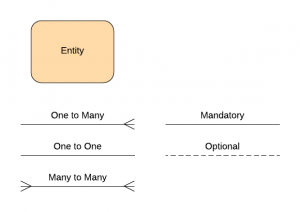
\includegraphics[width=\textwidth/5]{Assets/DB_ERD_01.png}
    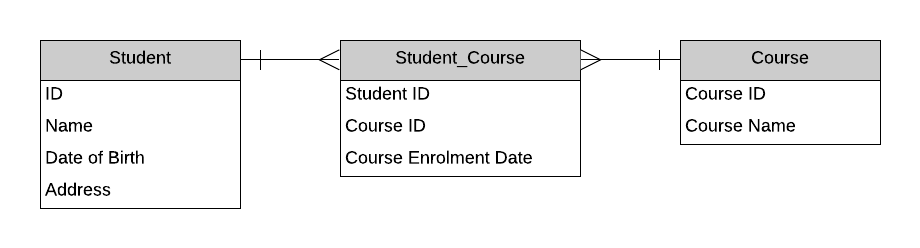
\includegraphics[width=\textwidth/5]{Assets/DB_ERD_02.png}

    \section{relationale Algebra}
    \scriptsize{
        $\sigma_{\{Datum=14.12.2017\}} (PRUEFUNG) \bowtie (\pi_{\{Matrikel, Name\}} (STUDENT))$
    }

    \section{Bereichskalkül}
    Bereichskalkül: $KUNDE(x,y,z)$ vs. Tupelkalkül: $KUNDE(k)$

    Ein Ausdruck hat die Form:$\{x1, x2, ... | \phi(x1, x2, ...)\}$
    \vspace{3mm}

    Beispiel: Kunden mit Bestellung

    $KUNDE(kdnr, kname, adresse, ort)$ und $AUFTRAG(auftragsnr, kdnr, warennr, menge)$

    Kunden mit Bestellung: $\{x,y,z| KUNDE(x,y,z,\_) \wedge AUFTRAG(\_,x,\_,\_)\}$

    \section{SQL Anfrage}
    \begin{lstlisting}[
        language=SQL,
        showspaces=false
     ]
     SELECT Matrikel, Name FROM Student WHERE Matrikel>2010;
    \end{lstlisting}

    \section{Integrität}
    \begin{description}
        \item[Nutzerdefinierte Domäne] eines Attributs, d.h. bestimmte Werte
        \item[Primärschlüssel PRIMARY KEY] nicht null, existiert und ist unique
        \item[Fremdschlüssel FOREIGN KEY] wie primary key aus anderer tabelle
        \item[CHECK-Bedingungen] werte vor insert prüfen
        \item[ASSERTIONs]
        \item[Trigger]
    \end{description}

    \section{CLOSURE-Algorithmus / RAP-Regeln}
    \begin{tabular}{c|c|l}
        R & Reflexivität  & $\{\} \Rightarrow X\rightarrow X$                                  \\
        A & Akkumulation  & $\{X\rightarrow YZ, Z\rightarrow AW\}\Rightarrow X\rightarrow YZA$ \\
        P & Projektivität & $\{X\rightarrow YZ\}\Rightarrow X\rightarrow Y$
    \end{tabular}

    \section{Normalformen}
    \begin{description*}
        \item[1.NF] Wertebereiche der Merkmale sind atomar (es gibt keine zusammengesetzten Werte).
        \item[2.NF] 1. NF + Nichtschlüsselmerkmale sind von allen Schlüsselmerkmalen voll funktional abhängig.
        \item[3.NF] 2. NF + kein Nichtschlüsselmerkmal ist von irgendeinem Schlüssel transitiv abhängig.
        \item[Boyce Codd] 3.NF + entgernen funktionaler Abhängigkeiten
        \item[4.NF] BC + Abhängigkeiten von mehrwertigen Attributmengen trivial und Attributmenge der Schlüsselkandidat
    \end{description*}


    \section{Konsultation}
    Mehrere theoretische Fragen? Nicht multiple choice wie in Moodle sondern zB Definitionen erklären (was ist Transaktion/Sicht?)

    ERD->Relationenschema
    bei 1:N Beziehung kommt Schlüssel von N Seite
    bei M:N Beziehung kommen Schlüssel von beiden Seiten
    bei 1:1 Beziehung kann Schlüssel von entweder einer oder der anderen seite gewählt werden


\end{multicols*}

\end{document}